\chapter{Analysis \& Design}
\myTop{In this chapter we analyze the requirements and design our sub-system for implementation.
We split our \subsystem{} into two sections, which are analyzed and designed separately in \secref{sec:virtualMeetingPlace} and \secref{sec:groupManagement}.
The complete architecture of \system{} is presented in \secref{sec:architecture}, and in \secref{sec:dbdesign} the database design of our \subsystem{} is presented.
This chapter makes a foundation for our sub-system and its implementation.}%
\label{chap:analysis}%
\label{chap:design}%
\label{chap:analdesign}%
The requirements from \secref{sec:requirements} are used in this chapter to analyze and design our \subsystem{}.
%One section being the usage of project groups, we call this part ``Virtual Meeting Place''.
%The other being the administration of project groups, called ``Project Group Management''.
%This division is corresponding to our division of end users in \secref{sec:enduser}.
%The analysis and design of each to part is presented in \secref{sec:virtualMeetingPlace} and \secref{sec:groupManagement} respectively.
Analysis and design is presented together for simplicity.



\section{Virtual Meeting Place}
\label{sec:virtualMeetingPlace}
\label{sec:projectgroup}
In this section we analyze the requirement Virtual Meeting Place.
Related requirements are: Navigate to Project Groups and Project Group Members.
These are analyzed in \secref{sub:designprojectgroupnavigation} and \secref{sub:projGrpMembers}.
%The following is an analysis of the requirement Virtual Meeting Place.

A virtual meeting place can take many forms.
As our requirement of a virtual meeting place states, we want it to comply with the Aalborg PBL model.
We analyze our requirements based on the conducted interviews and demo meetings and our own experiences.

We refer to the tools that our peer-groups develop as \detdeandrelaver{}s.
The aspects of the requirement Virtual Meeting Place that are presented here are: Structure of virtual meeting place, assignment of virtual meeting place, division of projects and groups, and virtual project tools integration.
These are presented below.


\subsection{Structure of the Virtual Meeting Place}
The members of a project group should have a place where they can meet and engage in project work using related \detdeandrelaver[]s.
Recall from \secref{sec:subSysDef} that our responsibility is to construct a place where this can happen, not construct the actual \detdeandrelaver[]s.
We have to decide the structure of the virtual meeting place.
%The two structures considered are described below.
We consider two different approaches, which are described below.
\pagebreak{}

\paragraph{Shared Group} One idea is to have every project group share everything with other project groups in a semester.
This corresponds to having every project group working in the same room in the real world.

\paragraph{Team Group} Another idea is to give a virtual group room to every project group and ensuring that only the members of the project group and the supervisors can contribute to the work on the project.
The corresponding situation in the real world is that every project group has their own group room where only they (and their supervisors) can do work on the project. \\

The Shared Group idea requires less effort than the Team Group idea to implement since no permissions need to be considered.
However, the Team Group is closer to the way that the Aalborg PBL model should work in practice.

We choose the Team Group structure. 
It is infeasible to have every project group share everything.
A project group member could be forced to look through a lot to find the relevant information to the given project group.
Furthermore, by allowing each project group to have their own virtual meeting place, the members can customize the place as they see fit by removing irrelevant tools and possibly adding new relevant tools.
The virtual place where these tools can be found is called the ``virtual group room''.
A virtual meeting place for a project group thereby consists of the virtual group room and the tools available.
This is illustrated on \figref{fig:projectgrouproom}.
\begin{figure}%
\center
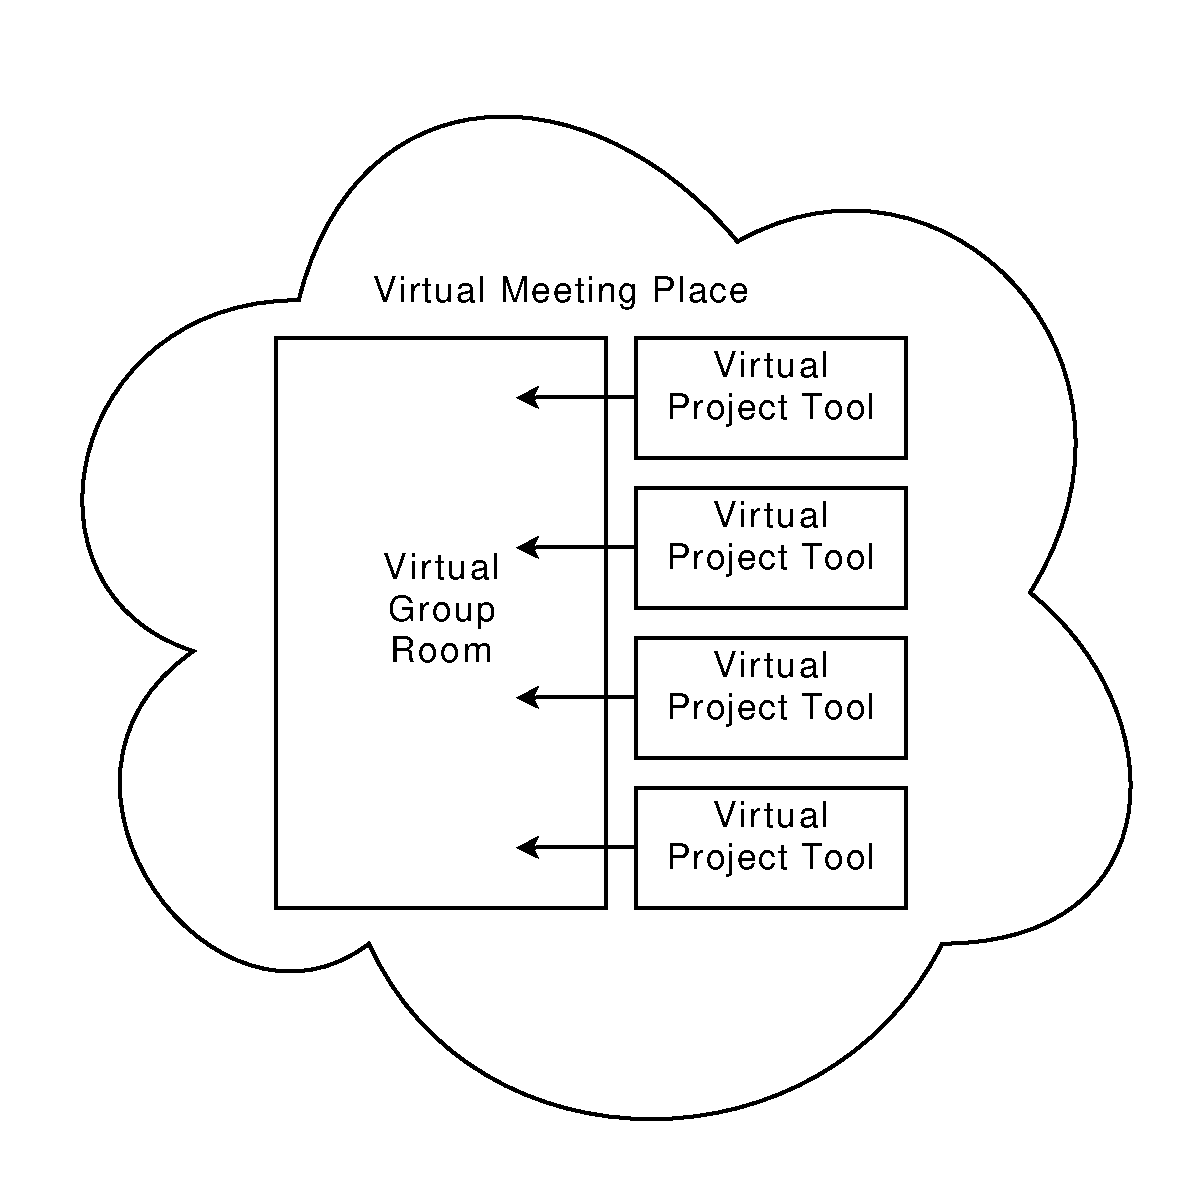
\includegraphics[scale=0.50]{images/VirtualMeetingPlace}%
\morscaption{The connection between the virtual meeting place and the virtual group room}%
\label{fig:projectgrouproom}%
\end{figure}
%For the rest of the report we refer to the virtual meeting place as the ``project group room''.

The virtual group room should have some of the same project related tools as a physical group room.
We as the \administrationgroup{} team implement the virtual group room, and the other three peer-groups implement the different tools.
%We as the \groupname{} implement the project group room, and the other three peer-groups implement the blocks (see \secref{subsec:blocks}) that provide different functionality.
%wrapper for the three other groups
%Joining of tools


\subsection{Assignment of Virtual Meeting Places}
At Aalborg University the physical group rooms are assigned to project groups periodically.
The period at which assignment of physical group rooms occur can differ.
Some of the most common periods are presented here:
\begin{itemize}
	\item \textbf{Never} There are no physical group rooms available because the field of study does not follow the Aalborg PBL model or the students are studying from remote locations.
	\item \textbf{Daily} The students have to reserve the physical group rooms on a daily basis (as stated in \appref{sec:jettePia}).
	\item \textbf{Half-yearly} Physical group rooms are assigned to each project group at the start of each semester.
\end{itemize} 

The virtual meeting place should be a hub where tools central to group work are available.
It should be similar to physical group rooms at Aalborg University in usage, and be available on a half-yearly basis.


\subsection{Division of Projects and Groups}
\label{sub:divProjGroup}
So far we have regarded project groups as an atomic entity, but projects and groups can be regarded as two different entities.
%In the Aalborg PBL model projects and teams exists as two different entities. 
The question arises if project groups should be designed as groups that have a relation to a project or as a single entity, where the group and project are one.
Below are the properties of the two variants presented.

%We will now list the properties of the two different variants. 

\paragraph{Groups and Projects Divided} 
\begin{itemize}
	%\item Projects and groups have a many-to-many relationship.
%	\item Directly reflects the objects of Aalborg PBL model. %Når jeg læser PBL Aalborg haløj ser jeg ikke hvorfor denne her passer bedst, der tager man jo udgangs punkt i et project/problem og dertil hører ét team, ikke flere teams.
	\item Flexibility between projects and groups, allowing many-to-many relationship.
	\item Complex to implement.
\end{itemize}


\paragraph{Groups and Projects United}
\begin{itemize}
	\item A group is linked to a single project; they are inseparable.
	\item Simple to implement.
\end{itemize}
%We will now examine related design options.

\begin{figure}[p]%
\centering
        \begin{subfigure}[b]{0.8\textwidth}
                \centering
                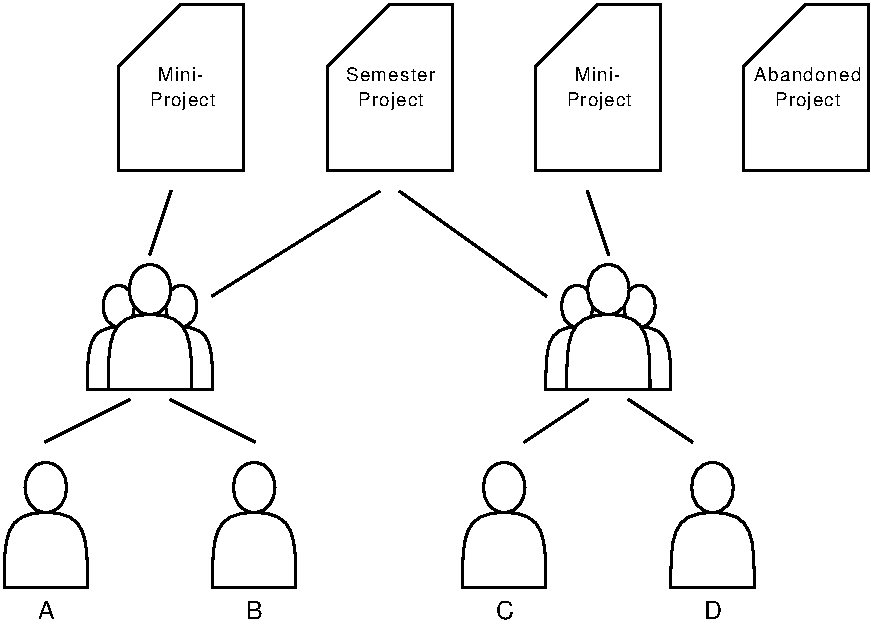
\includegraphics[width=\textwidth]{images/groupprojectdivision.pdf}
                \morscaption{Divided}
                \label{fig:divProjGroup:div}
        \end{subfigure}%
				\vspace{10mm}
        \begin{subfigure}[b]{0.8\textwidth}
                \centering
                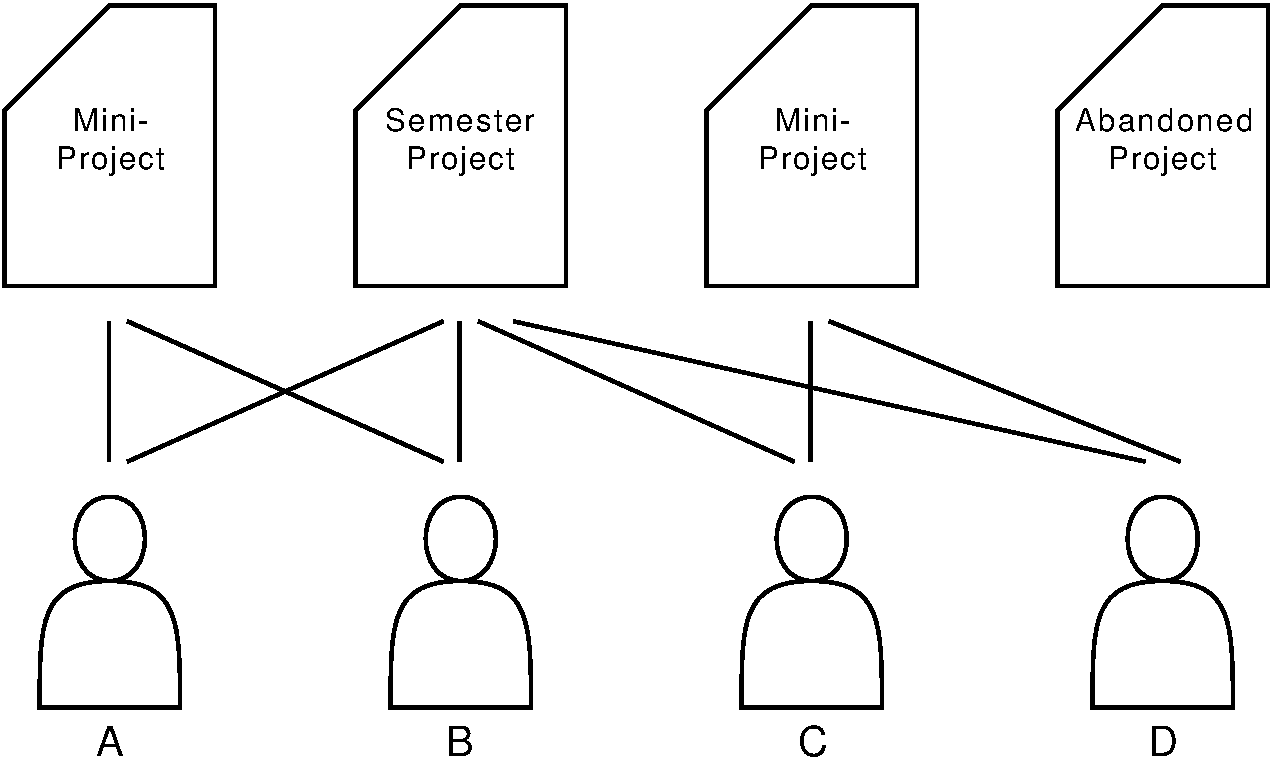
\includegraphics[width=\textwidth]{images/groupprojectunited.pdf}
                \morscaption{United}
                \label{fig:divProjGroup:united}
        \end{subfigure}%
\morscaption{The difference between the two approaches to the division of project and group illustrated by an example}%
\label{fig:divProjGroup}%
\end{figure}

The differences between these variants are illustrated with an example in \figref{fig:divProjGroup}.
The example is as follows:
There are four students identified by the letter A to D, and four projects; two mini projects, one semester project, and a single abandoned project.
Students A, B, C, and D collaborate on the semester project.
Students A and B are working on a mini project.
Students C and D are working on the other mini project.
Finally no one is working on the abandoned project.

Intuitively the option to divide groups and projects (seen in \figref{fig:divProjGroup:div}) might seem more appropriate since it introduces a level of indirection.
However, our interview with Lene (seen in \appref{sec:lene}) shows that the administrative personnel does not see any benefit from having any extra levels of indirection between students and projects.
%To select which of these divisions to choose we have contacted Lene W. Even and conducted an interview (seen in \appref{sec:lene}).
Since we are working agile we prefer to take the simplest viable approach and allow for extension of the system later.
We choose to design groups and projects as one entity (seen in \figref{fig:divProjGroup:united}) in accordance with the needs of our end users and to simplify our system.
The database design for storing project groups and members of the project group is found in \secref{sec:dbdesign}.
% -- note that we have not been in contacts with students for this decision.

\subsection{Virtual Project Tools Integration}
\label{sub:interActivities}
As mentioned previously we are developing a virtual group room where different \detdeandrelaver[]s can be used to perform project work.
The \detdeandrelaver[]s are primarily developed by our peer-groups.
For the \detdeandrelaver[]s to be available to the users through the virtual group room we have to have a common interface over which the virtual group room and the \detdeandrelaver[]s can communicate.
A typical communication message from the virtual group room to the \detdeandrelaver{} could be a request to make the tool render itself.
Alternatively we could integrate every tool directly into the virtual group room.
This, however, is not extensible enough.
Recall that we are four peer-groups of three to four students working together, which means that we would likely ``step on each others toes'' if we all were to work on the same component at the same time.
Furthermore, there is a group of students next year that must take over this project.
They might want to change the functionality or disable a tool.
This should be much easier if each tool is encapsulated in a component with a common interface than if every tool were intertwined in a single component.

Now that we have established that a there is a need for an interface between the \detdeandrelaver[]s and the virtual group room, we want to examine the possibilities that we have for doing so.
The two broad categories that the final choice can fall in are: Using an existing interface or developing a new interface.
These are not mutually exclusive.
We may take an existing interface and modify it to fit our needs.
Since we are making a plugin for an established LMS, we need to examine the possibilities in it to find an existing interface.
There are two plugin types in \moodle{} that we consider to be used as interface: \block{}s and activity modules.
Both of these are described in \secref{sub:plugins}.
By choosing any of these as the interface we restrict our peer-groups to make some or all of their \subsystem{} as the given plugin type, hence this is a joint decision.

%Intuitively the activity module might seem like the right choice, after all the name is \emph{activity} modules.
%However, activity modules are not for general \detdeandrelaver[]s, but only for course \detdeandrelaver[]s.
An activity module is required to have a database relation containing the instances of the activity module, each of which must have a link to a course~\cite{moodleactivitymodule}.
We do not use this idea because we do not want to have links between our project groups and courses -- a project group is an entity in its own right.

We now consider whether to use \block{}s or develop a new interface.
Developing a new interface would give us more freedom because we may choose exactly how it is defined.
On the other hand a \block{} ensures that \system{} will have a similar look and feel as the rest of \moodle{}.
Additionally, the students that take over next year will have accessible documentation through the \moodle{} Documentation about how to modify \detdeandrelaver[]s or add new ones.
The advantages of \block{}s outweigh the additional freedom that we may gain from defining our own interface.
This leads us to choose to use \block{} plugin type that every \detdeandrelaver{} must be implemented as.
For the virtual group room to communicate with \detdeandrelaver[]s it can use calls to member methods of \block{}s.
%E.g.\ to render a \block{} a call to \me{get\_content} is used~\cite{moodleblockapp}.
%\moodle{}, however, provides functionality to render all blocks associated with a given page.


\subsection{Navigation to Virtual Group Room}
\label{sub:designprojectgroupnavigation}
For a user to navigate to a virtual group room that he is a member of, there should be a procedure like the one for navigating to courses in which the user is enrolled.
To accomplish this we have looked at how navigation to courses work in \moodle{}.
There is currently a problem in Moodle when navigating to courses. 
When a user is enrolled in a large number of courses his entire front page is filled with links to those.
There is no built-in functionality to move or sort the links.
ELSA mentioned this problem during the meeting that we conducted with them described in \secref{sub:elsaInterview}.

We want to avoid this problem when we design the navigation for project groups.
Moodle has a navigation block with a list of important links.
We want to add an item to this list that, when expanded, shows the project groups the user is a member of.
Since a supervisor or an administrator might be a member of a many project groups, we want to limit the size of the list of project groups.
We do this by showing a maximum number of project groups according to a preset value.
If the user is a member of more project groups we show a link to a page that has a list of all the project groups that the user is a member of.


\subsection{Presentation of Members}
\label{sub:projGrpMembers}
Recall that the Presentation of Members requirement must ensure nearness for project group members.
If members of a project group tend to work in the same physical room, they have nearness.
To fulfill this requirement students conducting group work from remote sites should be able to experience nearness through our system.
The \supervisorgroup{} team has requested a feature for supervisors to see photographs of the members of a project group to help them identify a particular group.
We choose to design this feature to accommodate the requirement for project group members.
A part of the virtual group room should show all the members of the project group belonging to the room.
There should be a photography of the members to help identify them.
There is to be a functionality to hide or remove the members since students working in a physical group room might not need this and therefore prefer to focus on the other \detdeandrelaver[]s available in the virtual group room.

\subsection{Combining the Aspects}
In this section we combine the aspects discussed in the previous sections.
First and foremost there is a project group room where \detdeandrelaver[]s can be used directly or alternatively linked to.
Secondly there are all the \detdeandrelaver[]s that are not located directly in the virtual group room.
Only students and supervisor(s) associated with a project group are allowed to access the virtual group room of the given project group.
An exception to this is the administrative personnel, who have privileges to access and change any virtual group room.

Users are linked directly to project groups.
This reduces the complexity of the system at the cost of freedom.

Each \detdeandrelaver{} related to a virtual group room is implemented as a \block{}.
This allows for a well defined interface, which a virtual group room can use to communicate with the \detdeandrelaver[]s related to it.

To ensure familiar navigation for a user to his virtual group rooms, we extend the existing navigation menu of \moodle{}.
To avoid expanding the navigation menu out of proportions we limit the number of project groups that will be shown and provide an additional page where every project group belonging to a user can be found.

To provide a sense of nearness and to help supervisors recognize project groups, a simple tool is added to every virtual group room.
It can be hidden by users, if they do not need it.













\FloatBarrier
\section{Project Group Management}
\label{sec:groupManagement}
\label{sec:projectgroupadministration}
%From \secref{sec:virtualMeetingPlace} we know that we need a notion of projects or project groups.
%In either case instances projects or project groups must be created in the system in some way, as the requirement Manage Project Groups states in \secref{sec:requirements}.
%Other requirements considered in this section are: Find Project Group and Introduce Roles.
%\todo{I det her kapitel er der anvendt project group når der tales om Moodle og groups eller student groups når der tales IRL, %Sørg for det giver mening når du læser det igennem ellers så ret det.}
%\subsection{The Approaches} %% Very much working title
% Creation % Editing (Change of name and similar, add members) % Deletion
During the meetings with ELSA (see \secref{sub:elsaInterview}) and the \admpers{} we discovered three different approaches to manage the project groups: Automatic management through external application, manual management by administrative personnel, and management by students. 
We will now examine the approaches and choose the one we feel is the best solution.


\subsection{Automatic Management}
\label{sub:automanagement}
%% Automatic Creation(Proposed by ELSA) (Michael)
In this section an automatic group management approach is explored.  

%ELSA proposes that groups should be created automatically through an external system. 
Courses are created automatically on Moodle by ELSA.
%This technique is already used at Aalborg University to create courses. 
The courses are not populated automatically, but it still eases the work load for the \admpers{}.  
A similar approach can be used to create project groups from an external database containing the student groups. 

With automatic management through an external system it is necessary to synchronize Moodle with the external system in the case that the project groups are changed. 
If the data is input only in the external system a one-directional synchronization is needed, but if groups can be created, added, and deleted in Moodle a bidirectional synchronization service must be created. 
This service must be able to handle conflicts if changes are done at the external application and Moodle at the same time.

After an interview with Mikael of IST (see \appref{sec:mikael}) we discovered that Aalborg University does not have a single system containing the project groups.
Several systems exist and some of the systems are not online.
Each of these systems contain a fragment of the entire set of project groups at Aalborg University.
Furthermore, some departments do not keep official records of the project groups.
In an interview Mikael explained that not all the systems have an API from which the groups can be extracted, and he is working on an API for one of the systems.
%Without an API from which to extract the groups this approac. 



%%% Maintanance 


\subsection{Student Management}
\label{sub:studentmangement}
%% User- self-Creation  (Else talks about maintanance should be done by students)
In this section an approach which lets students create, edit, and delete project groups is discussed. 

In some cases the administrative personnel do not know which project groups are created (see \appref{sec:mikael}), and it is not guaranteed that all students want an online project group in Moodle. 
Therefore, a solution is to allow students to manage, by allowing them to create and edit their project groups as needed without adding extra workload to the administrative personnel.

The problem of this approach is that students might create badly named project groups or misuse the system by vandalizing the project groups of other students. 
This approach must include various security constraints to ensure proper use. 
Students should not be able to delete project groups they are not members of or to delete project groups by mistake. 
A mistaken deletion of a project group late in the semester could lead to a large amount of lost information and work. 
The creator of the project group must be able to govern who can be a member, or the members of the project group must accept new members.
Alternatively they should not be able to add or remove members from a project group after creation since a student should not be able to join a project group they do not belong to. 


\subsection{Administrative Personnel Management}
%% Administration personel creation (Lene creates courses and notes who is in the groups)
In this section the approach of having the administrative personnel manage project groups is discussed. 

The administrative personnel plays a central role in the administration of the courses and project groups of Aalborg University and is thereby capable of adding the necessary project groups to Moodle. 
Since the administrative personnel is trained professionals this approach ensures that only the needed project groups are created and that they are maintained properly. 
%That is with good naming convention.
A drawback to this approach is that it adds more work to the administrative personnel.

%\ \\ 

%----------------------------------------------------7\subsection{Design}
\subsection{Choosing an Approach}
The automatic management approach using an external system can be ruled out due to the fact that there does not exist a central project group database at Aalborg University, and the decentralized system at our department, AdmDB, is in the process of getting a new API developed.
Therefore the current API is going to be deprecated in the near future. 
If a centralized system with an API to extract project group information existed this would be the ideal approach, since it will not add workload to the administrative personnel and all project groups will exist in Moodle. 

From the two remaining approaches we choose to have the administrative personnel manage the project groups. 
We choose this because the student management approach has several constraints, which must be taken into account. 
With the student approach the administrative personnel must be able to clean up the project groups and therefore an administration panel for the \admpers{} is still necessary.
Without having to spend time figuring out how to constrain the system to prevent misuse, we can implement a working system by choosing the administrative personnel management approach.
The two approaches do not exclude each other, and the functionality used in the chosen approach can be reused if the other approach is implemented later.

With the chosen approach administrators need to be able to add, remove, and edit project groups.
Per default Moodle has a \block{} called Settings. 
If a user is an administrator there is a list in this block called Site administration. 
This list contains a lot of tools administrators use, and we choose to add project group administration to this list. 

We want a page where administrators can add a new project group that also adheres to Moodle standards.
It should be possible to name a group, add the desired members, and choose who the supervisors of the project groups are.

Additionally, there needs to be a list of all project groups.
From this list it should be possible to add, edit, and delete project groups. 
This list can potentiality grow very large, so there needs to be a way of finding a specific project group or a specific set of project groups as specified by the requirement Find Project Group.
This requirement is fulfilled by developing a filter system, where an administrative user can add filters on attributes to find a specific project group or a set of project groups.
The filter attributes should be those that administrative users are likely to use.
During the demo meeting described in \appref{sec:lenedemoone} we experienced that our end users need to find a project group based on its name.
This has lead us to decide that the project group name should be a filter attribute.

The final requirement we consider is Introduce Roles.
An administrative user must be able to set roles of the members of a project group.
We choose to allow an administrative user to change the role of a project group member in the page where he can add and remove members.
The roles that we consider to be important in a project group are student and supervisor.

An option we consider is to allow administrative personnel to create roles themselves, to adapt to a given situation.
However, we have not found any need for this, hence we choose only to have the two roles student and supervisor.







\section{Architecture}
\label{sec:architecture}
\system{} is an extension of \moodle{} and can be seen as a package of plugins. 
The architecture does not specify how each plugin should be created, but specifies a general structure of the components of the system. 
The complete architecture can be seen in \figref{fig:architecture}.
\begin{figure}[h!t]
	\centering
		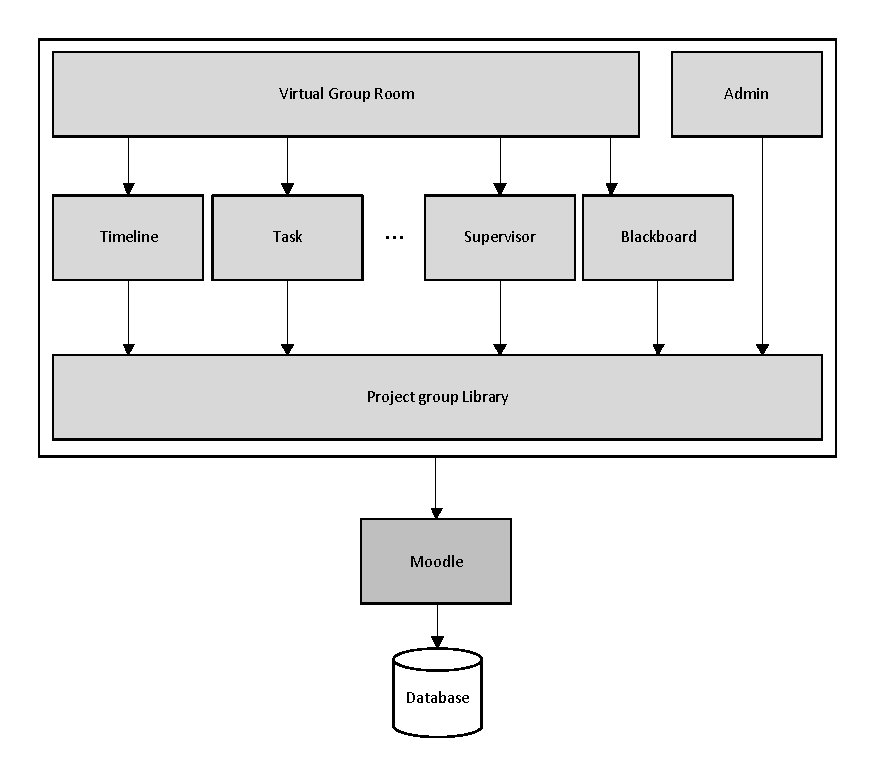
\includegraphics[width=\textwidth]{images/architecture.pdf}
	\morscaption{The overall architecture of MyMoodle}
	\label{fig:architecture}
\end{figure}

The architecture consists of a total of five layers. 
The three uppermost constitute \system{}, they have a common dependency, namely the Moodle platform. 
Layers four and five are Moodle and the Database system respectively.
%Our extension  as a plugin of Moodle and use functions supplied by Moodle to function.

We explain the three uppermost layers as:
\begin{enumerate}
	\item The uppermost layer is the virtual group room and the administration tool.
	%The virtual group room is used for presenting the virtual meeting place for a project group.
	The virtual group room is described in \secref{sec:virtualMeetingPlace}.
	The administrative tool is used by administrative personnel for managing project groups.
	It is described in \secref{sec:groupManagement}.
	This layer is called ``View Layer''.
	\item Directly below the uppermost layer is the middle layer, which consists of the four components: Timeline, Task, Supervisor, and Blackboard.
	These four components are created by our peer-groups and are not explained further.
	We call this layer ``Content Layer'', since the components in this layer generate content for the virtual group room component.
	This layer has three dots in the center in order to show that there exist more components and more can be added here. 
	%An example is the \detdeandrelaver{} that presents the members of the project group. 
	\item Below the Content Layer is the project group library, which contains common functionality.
	This layer handles all communication between the components in the Content Layer.  
	We call this layer the ``Library Layer''.
\end{enumerate}


There are two primary factors we need to consider when planning our architecture. 
Firstly, we are four sub-groups working together. 
This creates the need for a structured way of communicating between the different component and it lets every \subgroup{} know how their component is connected to the rest of the project. 
Secondly, the project should be passed on, which requires an architecture that grants great comprehensibility and extensibility of the project.
%alex -> <@:-D-|-<

It is not possible to make a strict layered architecture due to the Moodle dependency, and the administrative tool, which does not have to use the Content Layer, but depends directly on the project group library and \moodle{}.
We do, however, prohibit ourselves from accessing the database directly, by using the Moodle Database Layer (note that it is not a layer in our architecture) described in \secref{sec:moodleoplatformdbml}.
In \figref{fig:architecture} the dependency from the box encircling \system{} indicates that every component in \system{} depends on the \moodle{} component.
The \moodle{} component consists of the Database Layer as well as the Context System, Capabilities, etc.

%These considerations leads us to design the illustrated architecture in \figref{fig:architecture}.
Note that the relative size of the components do not imply anything, e.g.\ the Moodle component is code wise much larger, than all of the components in \system{} combined, but is illustrated with a rectangle the same size as any of the Content Layer components.














\section{Project Group}
\label{sec:projectgroup}
In this section the different aspects of the concept of the project groups will be described.
First we want to introduce the concept of a virtual meeting places for project groups.
How to navigate through the project groups is described afterwards.
Finally the design decisions regarding management of project groups is described.
\todo{Tjek igennem når analysen om dette emne er lavet }

\subsection{The Virtual Meeting Place}
The members of a project group should have a place where they can meet and engage in project related activities.
Recall from \secref{sec:subSysDef} that our responsibility is to construct a place where this can happen, not construct the actual activities -- that is the responsibility of our peer-groups.
We have to decide the scope of the virtual meeting place.
For example who should be able to see the work in progress of a project and who should be able to modify it.
One idea is to have every project share everything with other projects.
This corresponds to having every project group working in the same room in the real world.
Another idea is to give a virtual group room to every project group and ensuring that only the members of the project group and the supervisors can contribute to the work on the project.
The corresponding situation in the real world is that every project group has their own group room where only they (and there supervisors) can do work on the project.
The first idea is easier than the second to implement since no permissions need to be considered.
However, the second idea is closer to the way that Aalborg PBL is implemented -- with a team working together on the project as described in \secref{sub:aaupbl}.

We choose the second idea.
It is simply too infeasible to have every project group share everything.
A project group member could be forced to look through many functionalities to find the one relevant to the given project group.
Furthermore, by allowing each project group to have there own virtual group room, the members can customize the place as they see fit by removing irrelevant functionalities and possibly adding new relevant functionalities.
For the rest of the report we refer to the virtual group room simply as the ``project group room''.

The project group room should have some of the same functionality as a physical group room.
We as the \groupname{} implement the page, and the other three peer-groups implement the blocks (see \secref{subsec:blocks}) that serve as different functionality.
A good aspect of using blocks is that it is easy to manage which blocks should be shown and where they should be shown on the page.
The project group room is a place where students can exchange information among themselves and with their supervisor.

\subsection{Navigation}
\label{sub:designprojectgroupnavigation}
There is currently a problem in Moodle when it comes to navigation. 
When a user is enrolled in a large number of courses their entire front page is filled with links to those courses.
There is no built-in functionality to move or sort the links.
ELSA mentioned this problem during the meeting that we conducted with them described in \secref{sub:elsaInterview}.
%ref Lene
\todo{insert refs to interview with Lene. Hvorfor til Lene når det er ELSA der omtales?}

We want to avoid this problem when we design the navigation for project groups.
Moodle has a navigation block with a list of important links.
We want to add an item to this list that, when expanded, shows the project groups the user is a member of.
Since a supervisor or an administrator might be a member of a many project groups, we want to limit the size of the list of project groups.
We do this by showing at max a preset value, and if the user is a member of more groups we show a link to a page that has a list of all the users's group.

\subsection{Managing Project Groups}
\label{sec:s}
Administrators need to be able to add, remove, and edit project groups.
Per default Moodle has a block called Settings. 
If a user is an administrator there is a list in this block called site administration. 
This list contains a lot of tools administrators use, and it is only natural to add project group administration to this list. 

We want a page where administrators can add a new project group that also adheres to Moodle standards.
It should be possible to name a group, add the desired members, and choose who the supervisor(s) of the group is/are.

Additionally there needs to be a list of all project groups.
This list can potentiality grow very large, so there needs a way of finding a specific group or a specific set of groups. \todo{lene interview ref}
From this list it should be possible to add, edit, and delete groups. 

The project group administration should be implemented in such a way that it does not decrease the efficiency for the administrative personal compared to the old system. 
This measure can only be used in placed where an existing project group administration system is used.
\section{Database}
\label{sec:dbdesign}
In this section we will present the design of our database.
Our design will support the concepts that we have introduced, namely project groups and project group members.

Recall that we are designing to comply with a relational database, more specifically an SQL database as described in \secref{sub:constraints}.

\subsection{Project Group table}
\label{sub:dbProjectGroup}
A project group is an entity that consists of different elements.
How these elements are represented in the database is described here.
One core element is the project group members, this is described in \secref{sub:dbProjectGroupMembers}.
The other elements will be represented as fields in the \rel{projectgroup} relation.
%The reason for this is that a project group is an entity that has some attributes which we want to save persistent.

A project group must be identifiable by both human and computers.
To make a project group identifiable by humans we give it a short name that must be unique among other project groups.
The field that holds the short name in the project group relation is called \field{shortname}.
Initially it may seem that the short name could be used as a general identifier (both for humans and computers) since a short name is unique.
However, this name might be changed during the lifespan of a project group.
We much rather prefer an identifier that is constant for a project group to a avoid race conditions. 
%and violations of referential integrity
An example of a race condition in this system could be a user trying to access a project group with an identifier (the short name in this case) while another user is changing the short name of the group.
Should the short name be changed before the first user is trying to access the project group.
The request will fail because the identifier that he is holding is deprecated.

We choose to have a numeric auto-incrementing \field{id} field to identify the project groups.
This cannot be set or changed by the users of the system.
%Ultimately a databse administrator could change it directly in the database, but we cannot guard gainst this assuming the database administrator has super user privelges.
It is a Moodle guideline to have an auto-incrementing field as primary key~\cite{moodledb}.
We clearly obey this guideline by making \field{id} the primary key of \rel{projectgroup}.

One could argue that the numeric id field could be used as human identifier as well.
However, we deem it much easier for a humans to remember and associate an alphanumeric name with a particular project group than an arbitrary number.
In summary a project group has two identifiers; the numeric \field{id} and the alphanumeric \field{shortname}.
The former being the primary key of the relation.

To give a better description of a project group, we have an optional field called \field{longname}.
This field does not need to be unique, but only serves as a description for a project group.

To allow project groups to be ordered or filtered based on which semester (or another time-based constraint) they belong to we choose to have a timestamp field called \field{created}.
The value of this field is the Unix-timestamp at the time of the creation of the project group.

The four fields of \rel{projectgroup} are as follows.
\begin{itemize}
	\item \field{id} to identify the group.
	\item \field{shortname} to easily identify the group for humans.
	\item \field{longname} of the group, for a more descriptive name.
	\item \field{created} timestamp for a given project group.
\end{itemize}

An instance of \rel{projectgroup} with a single tuple (representing our own group) is shown \figref{fig:projectgrouprel}.
Notice in the figure that \field{shortname} might seem somewhat cryptic.
It translates to: ``Software Engineering, 6\ths{} semester, group number 8, spring (for\aa{}r), 2012''.
This illustrates the need for \field{longname}, since supervisors might find difficulty distinguishing several groups of the same semester simply by their group number.
\field{longname} gives a more descriptive name that should clearly give an idea of which it project group is.

\begin{figure}[htb]
	\centering
		\begin{tabular}{|l|l|p{0.5\textwidth}|l|}
			\hline
			\field{id} & \field{shortname} & \field{longname} & \field{created} \\
			\hline
			1 & SW608F12 & \groupname{} working on \system{} & 1337723013 \\
			\hline
		\end{tabular}
	\morscaption{Example of an instance of \rel{projectgroup}}
	\label{fig:projectgrouprel}
\end{figure}


\subsection{Project Group Members table}
\label{sub:dbProjectGroupMembers}
As opposed to a project group a project group member is not an entity in its own right.
A project group member is a user that is a member of a project group.
\moodle{} saves users in a relation named \rel{user}.
This relation contains information about the users of the system -- a unique identifier in particular -- and is part of the \moodle{} core database schema~\cite{moodledbschema}.
We want project group members to be represented in the database as a link between \rel{projectgroup} and \rel{user}.
We want this link to be many-to-many, since a project group can contain many members and a user can be a member of many project groups.

We can save the link in either \rel{user} or \rel{projectgroup}, or create a new relation to save them in.
We state in our system definition (seen in \secref{sec:systemDef}) that current functionality of \moodle{} should not be altered.
The first alternative is therefore out of the question since we cannot guarantee that the other parts of \moodle{} will continue to work as before if we alter in the core database relations.

Should we choose the second alternative we would make $n$ fields in \rel{projectgroup}, each containing a member of the project group or a value indicating no members, e.g. as null.
This would set a maximum of $n$ members on every project group.
If there is a maximum number of members that will ever be in a project group and this number is acceptably low this alternative might be viable.
%We do not, however, know any such number.
The number of users in the system could be a candidate for a maximum value.
This number may, however, change as more users are added to the system.
Furthermore, this number is likely to be larger than the actual maximum number of members in any group, assuming that no or few projects are conducted by every user of a \moodle{} system.
Another option is to choose a value that we believe is high enough for most purposes.
This would result in a many-to-$n$ link between project groups and users, in that a project group can have $n$ members and a user can be a member of any number of project groups.
If this $n$ value is chosen to high, space will be wasted, e.g. if $n$ is set to $20$ and no project group ever has more than 10 members, at least 10 fields in each \rel{projectrgoup} tuple will be wasted.
If $n$ is too low the system will be unacceptable because some desired project groups cannot be created.

The final alternative requires a new relation which stores a combination of users and project groups.
This allows for a true many-to-many link between users and project groups.
By choosing this alternative we have great extensibility, e.g. we are able to save the role of project group member in this relation as well.
A weakness to choosing this alternative is greater complexity by an increase in the number of relations.
The strengths of this alternative outweighs its weaknesses and it is better than the previous alternative by allowing a true many-to-many link without wasting space or making the system unacceptable.
Hence we choose this alternative as the way to save project group members in the database.
The relation that is used to link \rel{user} and \rel{projectgroup} is called \rel{projectgroup\_members}.

%%%%%%%%%%%%%%%%%%%%%%%%%%%%%%
% M�ske skal vi inds�tte en  %
% sub-subsection her         %
%%%%%%%%%%%%%%%%%%%%%%%%%%%%%%

For \rel{projectgroup\_members} to link \rel{user} and \rel{projectgroup} it will have a foreign key to both of these relations' primary keys.
The fields that hold these foreign keys are called \field{user} and \field{projectgroup} respectively.
The combination of \field{user} and \field{projectgroup} is a candidate key for \rel{projectgroup\_members}.
However, as with \rel{projectgroup} we choose to have a numeric auto-incrementing single field called \field{id} to comply with \moodle{} guidelines~\cite{moodledb}.
We still make the combination of \field{user} and \field{projectgroup} unique, to ensure that no person is a member of the same group more than once.

Whenever a user is a member of a project group we want to have a role associated to that member.
We can choose to give every user a role and whenever that user is a member of a project group he can act and have privileges as fit for the role.
Another way to do it is to save the role along with the link between users and project groups.
We prefer the latter for two reasons.
Firstly a user may have different roles in different project groups, e.g. a Ph.D. student has a student role in his Ph.D. project, but may also be supervising projects being conducted by younger students.
Secondly we would have to make a new relation to contain only this information and thus increase complexity if the former alternative is to be chosen.
We will not alter the core relations such as \rel{user}, as described in \secref{sub:dbProjectGroup}.

To allow for extensibility we save the creation and update time of each tuple in \rel{projectgroup\_members} in \field{created} and \field{updated} respectively.
It may be useful to have these timestamps for administrative personnel, e.g. to see whether or not a user has joined a project group later than the other members.

The final set of fields in \rel{projectgroup\_members} are:
\begin{itemize}
	\item \field{id} which is Moodle convention. \cite{moodledb}.
	\item \field{projectgroup} references to the related project group.
	\item \field{user} references to the related user.
	\item \field{role} denoting the type of membership the user has to the group.
	\item \field{created} is the timestamp for its creation.
	\item \field{updated} is the timestamp for the last update to the membership. 
\end{itemize}

\figref{fig:projectgroupmembersrel} shows an instance of \rel{projectgroup\_members} containing four students (indicated by role ``0'') and a supervisor (indicated by role ``1'').
Notice that all tuples have the same \field{projectgroup} value.
This indicates that every tuple links user to the same project group, namely the one shown in \figref{fig:projectgrouprel}.

\begin{figure}[htb]
	\centering
		\begin{tabular}{|l|l|l|l|l|l|}
			\hline
			\field{id} & \field{projectgroup} & \field{user} & \field{role} & \field{created} & \field{updated} \\
			\hline
			1 & 1 & 1 & 0 & 1337723013 & 1337723013 \\
			\hline
			2 & 1 & 2 & 0 & 1337723013 & 1337723013 \\
			\hline
			3 & 1 & 3 & 0 & 1337723013 & 1337723013 \\
			\hline
			4 & 1 & 4 & 0 & 1337723013 & 1337723013 \\
			\hline
			5 & 1 & 17 & 1 & 1337723184 & 1337723184 \\
			\hline
		\end{tabular}
	\morscaption{Example of an instance of \rel{projectgroup\_members}}
	\label{fig:projectgroupmembersrel}
\end{figure}


The database scheme can be seen in~\figref{fig:projectgroupsdb}. 
The user entity is a built-in part of Moodle and is not modeled by us. 
\begin{figure}
	\centering
		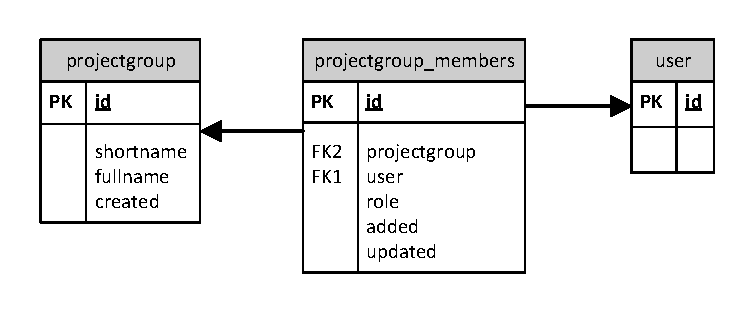
\includegraphics[width=\textwidth]{images/projectgroupsdb.pdf}
	\morscaption{The database scheme of project groups and memberships.
	Most of the data fields of the user table are omitted for brevity.
	The user table consist of more than 50 fields}
	\label{fig:projectgroupsdb}
\end{figure}

%To test the scheme for redundancy we check to see that the scheme conforms to boyce-codd normal form (BCNF). To check this we 

